\documentclass[11pt]{article}

\usepackage{graphicx}
\usepackage{url,apacite} 

\newcommand{\numpy}{{\tt numpy}}    % tt font for numpy
\topmargin -1in
\textheight 9in
\oddsidemargin -.25in
\evensidemargin -.25in
\textwidth 7in

\begin{document}

\author{Anto´nio Almeida, UP2015058365}
\date{May $10^{th}$, 2019}
\title{Paper Summary - The Multiple Sequence Alignment Problem in Biology}
\maketitle


% \medskip

\section{Introduction}

This report consists of a summary of the paper \textit{The Multiple Sequence Alignment Problem}\cite{Carrillo:1988:MSA:53867.53874}, as part of a project for FCUP's course Algorithms for Bioinformatics\footnote{https://sigarra.up.pt/fcup/en/ucurr\_geral.ficha\_uc\_view?pv\_ocorrencia\_id=430165}. This paper was selected because it has an important historic role on the field of Bioinformatics, and its content aligns well with the goals of the course.

\section{Summary}

\subsection{Introduction}

Character sequence comparison is common and useful throughout multiple fields such as molecular biology, speech recognition, and computer science. It is particularly important in molecular biology through the form of sequence alignment, where it has been critical in the study of evolution and genetics. 

Considering the problem of comparing two related proteins, i.e., sequences composed of an alphabet of twenty amino acids, in the course of divergence from a common ancestor, mutations may occur through the form of replacements, insertions, and deletion of amino acids. Recreating the original correspondence of amino acids consists of considering all possible transformations of the sequences and choosing a configuration that is optimal. 

Additionally, in problems such as the construction of an evolutionary tree based on sequence data, or in protein engineering, a molecular biologist must compare more than two sequences simultaneously, i.e., must perform multiple sequence alignment.

Dynamic programming methods have proven to be useful in solving the optimization problems associated with sequence comparison, despite the great rise in complexity with dimension. 

In the following sections, we'll be presenting simplified versions of the formal definitions of concepts related to the multiple sequence alignment problem, followed by a discussion on the same topic.

\subsection{Sequences}

Assuming an alphabet $\alpha$ of $n$ characters, i.e.,  $$\alpha = \big\{ \alpha_1, ... , \alpha_n \big\}$$

A $sequence$ of $k$ characters, or a $k-sequence$ $S$ is a set of the form $$S = \big( \alpha_n1, \dots , \alpha_n_k \big)$$, where for each $j = 1, \dots  , k$, $n_j$ is a natural number such that $1 \leq n_j \leq n$.

Alongside $\alpha$, let's consider another alphabet $\beta$ which is obtained from $\alpha$ by adding the blank character "$-$", i.e., $$\beta = \big\{ - \big\} \cup \big\{ \alpha_1, \dots , \alpha_n \big\}$$

\subsection{Alignments}

An $alignment$ of the sequences $S_1, \dots , S_n$ is another set of sequences $\overline{S_1}, \dots, \overline{S_n}$ such that each sequence $\overline{S_i}$ is obtained from $S_i$ by inserting blanks in positions where some of the other sequences have a nonblank character.

Each alignment of the sequences $S_1, \dots , S_n$ encodes a set of different insertions, deletions, and replacements that transform one sequence into another. 

For an ilustration of the notion of an alignment, let's consider the short amino acid sequences, $$S_1 = DQLF, S_2=DNVQ, S_3=QGL$$ where each capital letter corresponds to a different amino acid. A possible alignment of these sequences is shown in Fig. \ref{fig:alignment}.

\begin{figure}
    \centering
    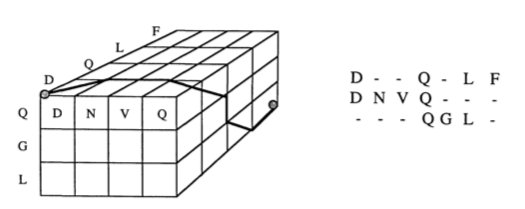
\includegraphics[scale=0.5]{alignment-example.png}
    \caption{An illustration of multiple sequence alignment on a three dimensional lattice.}
    \label{fig:alignment}
\end{figure}

\subsection{Paths}

To any given set of $N$ sequences $S_1, \dots , S_n$, of length $k_1, \dots , k_n$, we'll associate a $lattice$ $L \big( S_1, \dots, S_n \big) $ in N-dimensional space. This lattice consists of the N-dimensional hypercubes resulting from the Cartesian product of $N$ strings of squares. Each of this strings represents a particular sentence and has as many squares as characters in the sequence. 

A $path$ $\gamma \big(S_1, \dots , S_n \big)$ between the sequences $S_1, \dots , S_n$ is a connected broken line joining the $original$ $corner$, corresponding to the first character of all sequences, to the $end corner$, corresponding to the last character of all sequences. At each step of this broken line, starting from the original corner, the correspondent point gets closer to the end corner. Paths in an N-dimensional lattice encode alignments of the N sequences that form the lattice. Additionally, each path is associated with a unique alignment.

A path in an N-dimensional lattice, $\gamma \big(S_1, \dots , S_n \big)$, can be projected into any of the planes formed by each pair of sequences $\big(S_i, S_j\big)$. The projected path, $p_ij\big(\gamma\big(S_1, \dots, S_n\big)\big)$, represents an alignment of the sequences $S_i$ and $S_j$.

\subsection{Optimal Paths}

If we define an set of scoring rules that penalize each individual deletion, insertion, or replacement, then we may assign a score to a given alignment corresponding to the sum of the scores of each of the transformations. There are multiple ways in which scoring rules can be established. The penalty for a particular transformation might be dependent on the position where it occurs and on the transformations it succeeds. 

The scoring rules allow us to assign to any given path $\gamma\big(S_1, \dots, S_n\big)$ a $measure$, $M\big(\gamma\big)$. The $M\big(\gamma\big)$ is a measure of the similarity among the sequences $S_1, \dots, S_n$, when they are compared according to the alignment associated to the path $\gamma$. 

Corresponding to each measure $M\big(\gamma\big)$ there is at least one path, $\gamma^*\big(S_1, \dots, S_n\big)$, such that $M$ attains a minimum value at $\gamma^*$. Such path is called an \textit{optimal path}. Optimal paths in a lattice $L\big(S_1, \dots, S_n\big)$ can be found by dynamic programming methods.

\subsection{Constraints on Multiple Alignments}

In this section, some observations are made on the problem of determining $\gamma^*\big(S_1,\dots,S_n\big)$ where $N > 2$, that will result in significantly fewer computations. The explanation is particularly formal and verbose. For simplicity, we will attempt to summarize the key conclusions, rather than the method to obtain them.

Considering any N-dimensional path $\gamma^e$ that will be called \textit{y-estimated}, then, $$M\big(\gamma^e\big) - M\big(\gamma^*\big) \geq 0$$.

Developing on this expression, for each $k,l = 1,\dots, N$, we can define a positive number $U_{kl}$ as an upper bound for the measure of the projection of any N-dimensional optimal path into the plane determined by the sequences $S_k$ and $S_l$. Then, when looking for $\gamma^*$ we need only consider paths $\gamma$ in $L\big(S_1, \dots, S_n\big)$ that satisfy $u_{kl}\big(p_{kl}\big(\gamma\big)\big) \leq U_{kl}$, $u$ being a function of the comparison score between a given pair of sequences. 

Based on this, we can define a set of paths $X$ as the only possible candidates to be an optimal path. To consider only paths in X means to execute the procedure to find $\gamma^*$ only in some subregion $Y$ of $L(S_1,\dots,S_n\big)$. Instead of applying the dynamic programming method to the entire lattice, it suffices to consider just the subregion $Y$. The regions $Y_{ij}$ can be determined using a simple variation of the base dynamic programming method. 

\subsection{Estimated Paths}

The smaller the region $Y$, the smaller the amount of computation necessary to find an optimal path. To obtain a small region Y we would need to produce an estimated path $\gamma^e$ with measure close to the measure of an optimal path. 

One approach to deal with this problem is based on the following observation: considering $\gamma^*_{ij}$ denotes an optimal path on the lattice $L\big(S_i, S_j\big)$, if there is a path $\gamma$ such that $p_{ij} = \gamma^e_{ij}$ for all $i,j$, then $\gamma$ is an optimal path for the N-dimensional problem. The idea is to construct $\gamma^e$ in such a way that its projections $p_{ij}\big(\gamma^e\big)$ are as close as possible to the optimal paths $\gamma^*_{ij}$.

Another approach is to start with a guess of an estimated measure $M^e$ which, unlike $M\big(\gamma^e\big)$, may not necessarily correspond to the measure of an actual $\gamma$. We then determine all upper bounds using $M^e$ and proceed to compute an "optimal" path $\gamma^{e^*}$ derived from the initial estimate. Then, if $M\big(\gamma^{e^*}\big)$, $\gamma^{e^*}$ is a true optimal path.

\subsection{Discussion}

Although the demonstrations presented were on the case where the lower dimension was two, the results may be generalized for any dimension less than N. The relationship between the alignment of N sequences and the problem of aligning subsets of these sequences an be exploited to develop multiple alignment algorithms with reduced computational requirements. It is clear that said algorithms would be a function of the size of the subregion $Y$ in the lattice $L\big(S_1, \dots, S_n\big)$ plus the number of computations necessary to generate it.

Additionally, further computational improvements may be achieved by noting that not all points in the subregion $Y$ must be stored in the computation of an optimal path.

Ukkonen has described a method for decreasing the computational cost of pairwise alignments when the measure of distance is very simple, e.g., identities have distance zero, all other transformations have a distance of one.

If the sequences to be compared differ by only a very few insertions, deletions, and replacements, a generalized Ukkonen algorithm would have computational advantages over an algorithm based on the aforementioned observations. However, Ukkonen's method becomes quite complicated and less efficient with more realistic measures of distance.

These results approach the N sequence multiple alignment problem as finding an $n$-dimensional path whose projections are optimal. Understanding the new forms of the problem suggested by this view can lead to more efficient algorithms, and to variants of the original problem which may have useful applications.

\section{Conclusion}
       
The paper studied proved itself to be a valuable read and focus of study, despite its heavy reliance on formal definitions ressions to arrive at its observations. While summarizing the most important observations and explanations provided, the word limit was significantly exceeded. An effort was made to reduce word count, yet the report's author believes it was a necessary tradeoff as to not oversimplify important concepts. The author is satisfied with the results and has learned a lot on the subject of multiple sequence alignment throughout the project.

\bibliographystyle{apacite} % We choose the "plain" reference style
\bibliography{refs} % Entries are in the "refs.bib" file

\end{document}
\grid
\grid